\section{Fordeling af besvarelserne}
\label{TestAfSkalaFordelingAfBesvarelserne}
%
Fra dette afsnit laves en henvisning til dokumentet med oversigten over fordelingen af besvarelser for besvarelserne til hver af skalaerne. (Som kommer til at ligge i elektronisk bilag)
%
\begin{figure}[H]
\centering
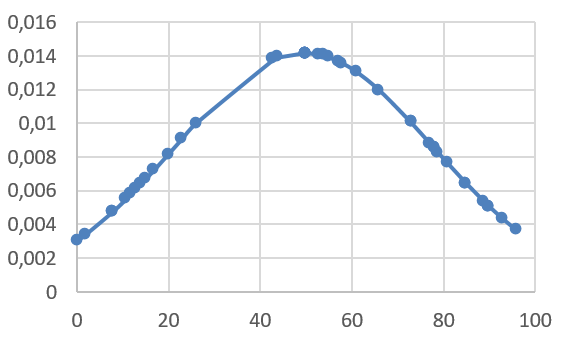
\includegraphics[width = 0.8\textwidth]{Figure/DatabehandlingSkalaer/FordelingSkala1} 
\caption{Fordelingen af besvarelserne til Scale Question 1 ``Hvordan synes du skærmen reagerede? '' (Ekstremt dårligt/Ekstremt godt)}
\label{fig:FordelingSkala1}
\end{figure}
\noindent
%
Det fremgår ret tydeligt, at skærmen ikke har reageret godt for alle, hvilket stemmer overens med vores observationer. Data fordeler sig groft i tre grupper: 0-30, 40-70 og 70-100.

